% =====================================================================
\chapter{Cointégration appliquée : sélectionner les paires sans se mentir}
\label{ch:7}
% =====================================================================

\section{Objectifs et organisation du chapitre}

\paragraph{Objectifs.} Le chapitre~4 a donné les tests de cointégration pour \emph{une} paire. En pratique, on teste des centaines ou des milliers de paires candidates, et c'est là que la plupart des stratégies échouent : on retient surtout des faux positifs. À la fin de ce chapitre, vous saurez : (1) quantifier le nombre de faux positifs d'une recherche de paires ; (2) appliquer les corrections de Bonferroni et de Benjamini-Hochberg ; (3) construire un pipeline de sélection qui combine a priori économique, test statistique et filtres de dynamique \citep{vidyamurthy2004,huck2009,krauss2017survey} ; (4) mesurer la performance hors échantillon des paires retenues ; (5) choisir entre ratio de couverture statique et glissant.

\paragraph{Code.} \texttt{code/ch07/ch07\_cointegration\_selection.py}, univers \texttt{code/common/universe.py}.

% =====================================================================
\section{Le problème des tests multiples}
% =====================================================================

\subsection{Combien de faux positifs ?}

Avec $N$ actions, il y a $m = N(N-1)/2$ paires. Si l'on teste chacune au seuil $\alpha$ et qu'aucune n'est cointégrée, le nombre de rejets suit à peu près une loi binomiale de paramètres $(m,\alpha)$ : on attend $m\alpha$ faux positifs. Pour $N = 100$, $m = 4\,950$ et $\alpha = 5\,\%$, cela fait environ 250 \og paires cointégrées\fg{} purement fortuites.

\begin{intuition}
Lancez 4\,950 pièces de monnaie dix fois chacune : quelques-unes tomberont huit ou neuf fois sur pile. Ce ne sont pas des pièces truquées, ce sont les plus chanceuses. Si vous les \og sélectionnez\fg{} pour les relancer, elles retomberont à la moyenne. Une paire qui a passé le test par chance se comporte de même hors échantillon.
\end{intuition}

\subsection{Deux façons de contrôler l'erreur}

\begin{definition}
Parmi $m$ tests, on note $V$ le nombre de faux positifs (hypothèses nulles vraies rejetées) et $R$ le nombre total de rejets.
\begin{itemize}
\item Le \emph{taux d'erreur par famille} (FWER) est $\Prob(V\ge1)$ : la probabilité de commettre au moins une fausse découverte.
\item Le \emph{taux de fausses découvertes} (FDR) est $\E[V/\max(R,1)]$ : la proportion attendue de fausses découvertes parmi les découvertes.
\end{itemize}
\end{definition}

\begin{proposition}[Bonferroni]
Si l'on rejette chaque hypothèse dont la $p$-valeur est inférieure à $\alpha/m$, alors $\mathrm{FWER}\le\alpha$, quelle que soit la dépendance entre les tests.
\end{proposition}
\begin{proof}
Soit $I_0$ l'ensemble des hypothèses nulles vraies, de taille $m_0\le m$. Sous une hypothèse nulle vraie, $\Prob(p_i\le\alpha/m) \le \alpha/m$ (propriété d'une $p$-valeur valide). Par l'inégalité de la réunion, $\Prob(V\ge1) = \Prob\big(\bigcup_{i\in I_0}\{p_i\le\alpha/m\}\big) \le \sum_{i\in I_0}\alpha/m = m_0\alpha/m \le \alpha$.
\end{proof}

Bonferroni est très conservateur : avec 4\,950 tests, il exige $p < 10^{-5}$. La procédure de Benjamini-Hochberg contrôle plutôt la proportion de fausses découvertes, ce qui convient mieux à une recherche de paires (on accepte quelques erreurs si la plupart des paires retenues sont bonnes).

\paragraph{Procédure de Benjamini-Hochberg (BH).} On ordonne les $p$-valeurs $p_{(1)}\le p_{(2)}\le\dots\le p_{(m)}$, on cherche le plus grand $k$ tel que $p_{(k)}\le kq/m$, et l'on rejette les $k$ hypothèses correspondantes. Sous indépendance des tests (ou une forme de dépendance positive), cette procédure garantit $\mathrm{FDR}\le q$.

\begin{pitfall}
Les tests de cointégration d'un même univers sont fortement dépendants : deux paires qui partagent une action, ou deux actions du même secteur, ont des statistiques corrélées. Les garanties théoriques de BH ne sont alors qu'approximatives. Surtout, \emph{toute} la recherche compte : si vous avez essayé trois fenêtres, deux sens de régression et deux spécifications de tendance, vous avez fait douze fois plus de tests que vous ne le pensez.
\end{pitfall}

% =====================================================================
\section{Un pipeline de sélection}
% =====================================================================

La littérature et la pratique convergent vers une sélection en plusieurs filtres, du moins coûteux au plus exigeant :
\begin{enumerate}
\item \textbf{A priori économique.} Restreindre les candidats aux actifs qui ont une raison de rester liés : même secteur ou sous-secteur, même sous-jacent, relation contractuelle (ETF et panier, deux catégories d'actions d'une même société). Cela réduit $m$ d'un facteur 5 à 50 et élimine les relations purement fortuites.
\item \textbf{Test de cointégration} (Engle-Granger dans les deux sens, ou Johansen), avec correction des tests multiples.
\item \textbf{Filtres de dynamique.} Demi-vie dans une plage exploitable (assez courte pour trader, assez longue pour couvrir les coûts) ; amplitude de l'écart suffisante par rapport aux coûts (chapitre~5) ; nombre de croisements de la moyenne.
\item \textbf{Stabilité.} La relation est-elle détectée sur plusieurs sous-périodes ? Le ratio de couverture est-il stable ?
\item \textbf{Contraintes pratiques.} Liquidité des deux jambes, disponibilité et coût de l'emprunt de titres pour la vente à découvert, frais.
\end{enumerate}

% =====================================================================
\section{Expérience : 4\,950 paires, 10 vraies}
% =====================================================================

On reprend l'univers simulé du chapitre~6 (100 actions, 5 secteurs, 10 paires réellement cointégrées) avec une formation de 500 jours et un trading hors échantillon de 250 jours (règle \emph{z-score} du chapitre~1, entrée à $\pm2$, sortie à 0, coûts de 5 pb par jambe). On distingue trois sortes de paires : les \emph{vraies} paires ; les paires \emph{partiellement liées}, dont une jambe appartient à une vraie paire (leur écart contient la moitié de l'écart stationnaire de la vraie paire, comme dans la cointégration partielle du chapitre~4) ; les paires \emph{sans lien}, dont l'écart est une martingale. Deux scénarios : vraies paires de demi-vie 4,3 jours ($\varphi = 0{,}85$) ou 13,5 jours ($\varphi = 0{,}95$). Douze univers par scénario.

\begin{table}[h]
\centering\small
\caption{Paires retenues par univers (moyenne sur 12 univers), selon la règle de sélection.}
\label{c7:tab:sel}
\begin{tabular}{lccccc}
\toprule
 & \multicolumn{2}{c}{Demi-vie 4,3 j} & & \multicolumn{2}{c}{Demi-vie 13,5 j}\\
\cmidrule{2-3}\cmidrule{5-6}
Règle & vraies & fausses & & vraies & fausses \\
\midrule
$p<5\,\%$ (4\,950 tests) & 10,0 & 265,2 & & 8,4 & 264,3 \\
Bonferroni & 9,0 & 0,0 & & 0,1 & 0,0 \\
Benjamini-Hochberg, $q = 5\,\%$ & 10,0 & 0,9 & & 0,1 & 0,0 \\
Même secteur (950 tests) $+$ BH & 10,0 & 0,7 & & 0,3 & 0,1 \\
\bottomrule
\end{tabular}
\end{table}

\begin{codebox}[ — E1 et E2, sélection et performance hors échantillon]
\textbf{Sélection} (tableau~\ref{c7:tab:sel}) : sans correction, 96\,\% des paires retenues sont fausses. Avec BH, presque toutes sont vraies \emph{si} le retour à la moyenne est rapide ; si la demi-vie est de 13,5 jours, 500 jours de formation ne suffisent plus à franchir le seuil corrigé et l'on ne retient presque rien. \textbf{Rendement hors échantillon par paire} (250 jours, en \% du notionnel brut, moyenne des moyennes par univers $\pm$ erreur-type entre univers, scénario 4,3 j) : vraies paires $3{,}71 \pm 0{,}14$ ; paires partiellement liées $3{,}49 \pm 1{,}93$ ; paires sans lien $1{,}69 \pm 1{,}61$. Les moyennes par univers des paires sans lien vont de $-4{,}5\,\%$ à $+13{,}1\,\%$, celles des paires partiellement liées de $-7{,}6\,\%$ à $+17{,}2\,\%$, celles des vraies paires de $3{,}0\,\%$ à $4{,}6\,\%$.
\end{codebox}

\begin{figure}[h]
\centering
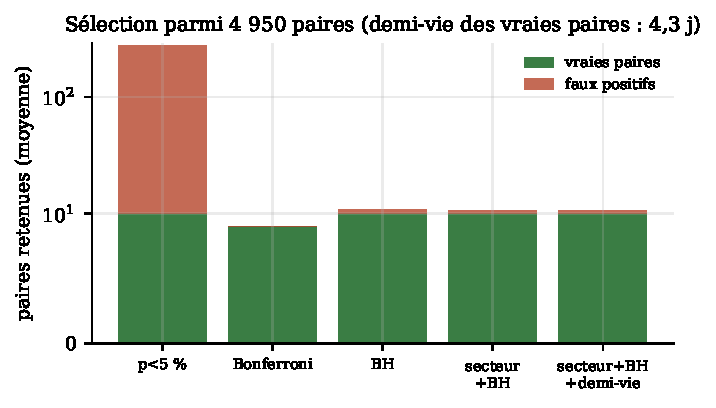
\includegraphics[width=0.7\textwidth]{ch07/selection_faux_positifs.pdf}
\caption{Paires retenues par univers selon la règle (échelle logarithmique au-delà de 10). Sans correction, les vraies paires (vert) sont noyées sous les faux positifs (rouge).}
\label{c7:fig:sel}
\end{figure}

\paragraph{Trois leçons.}
\begin{enumerate}
\item \textbf{Les faux positifs ne perdent pas forcément d'argent en moyenne, ils ajoutent du risque.} Une paire sans lien a une espérance de gain nulle (l'écart est une martingale), mais une variance énorme : la moyenne d'un univers à l'autre oscille entre $-4{,}5$ et $+13{,}1\,\%$. Une petite moyenne positive sur un échantillon n'est pas une preuve. Remarquez aussi que l'erreur-type \og naïve\fg, qui traite les paires comme indépendantes, vaut $0{,}36\,\%$ alors que l'erreur-type correcte entre univers vaut $1{,}61\,\%$ : des paires qui partagent des actions ne sont pas des observations indépendantes.
\item \textbf{Les relations partielles existent et rapportent, mais de façon instable.} Les paires partiellement liées gagnent en moyenne autant que les vraies, avec une dispersion entre univers environ quatorze fois plus grande.
\item \textbf{La correction a un prix : la puissance.} Quand la demi-vie est longue, la correction pour tests multiples supprime aussi les vraies paires. Il faut alors plus d'historique, des données plus fréquentes si la dynamique le permet, ou un a priori économique plus serré qui réduit le nombre de tests.
\end{enumerate}

\begin{codebox}[ — E3, persistance des paires retenues]
Parmi les 131 paires retenues par BH (scénario 4,3 j, 12 univers), 122 sont de nouveau cointégrées à 5\,\% sur la fenêtre suivante (décalée de 250 jours), dont 120 vraies. La stabilité dans le temps est un excellent filtre complémentaire : une relation réelle se retrouve d'une fenêtre à l'autre.
\end{codebox}

% =====================================================================
\section{Ratio de couverture : statique ou glissant ?}
% =====================================================================

Une fois la paire retenue, faut-il garder le $\hat\beta$ estimé sur la formation ou le réestimer en continu sur une fenêtre glissante ? Une fenêtre glissante s'adapte aux changements, mais chaque réestimation sur peu de données ajoute du bruit, et ce bruit se transforme en P\&L parasite : l'écart \og bouge\fg{} parce que $\beta$ bouge, pas parce que les prix ont bougé.

\begin{codebox}[ — E4, erreur sur le ratio quand le vrai ratio est constant]
Erreur absolue moyenne sur $\beta$ (vrai $\beta = 1$, 30 vraies paires) : statique sur 500 jours $0{,}026$ ; glissant sur 250 jours $0{,}033$ ; glissant sur 60 jours $0{,}073$.
\end{codebox}

Quand la relation est stable, la fenêtre glissante courte est presque trois fois moins précise. Elle ne se justifie que si le ratio change réellement ; et dans ce cas, le filtre de Kalman du chapitre~8 fait le même travail de façon optimale, en dosant automatiquement la réactivité.

% =====================================================================
\section{Dimensionner les positions}
% =====================================================================

Pour que chaque paire contribue au risque de façon comparable, on dimensionne la position par la volatilité de l'écart plutôt qu'en montant fixe : si l'écart (en log) a un écart-type quotidien $\sigma_S$, une position de notionnel $K$ sur la jambe $Y$ a un risque quotidien d'environ $K\sigma_S$. Viser un risque cible $R$ par paire donne $K = R/\sigma_S$. On limite ensuite le notionnel total, l'exposition par secteur et l'exposition au facteur de marché résiduel (si $\hat\beta$ diffère des expositions réelles au marché, la paire n'est pas neutre). Le chapitre~17 traite le dimensionnement global.

% =====================================================================
\section{Ce que la théorie apporte, et ses limites}
% =====================================================================

\paragraph{Apports.} Un cadre pour savoir combien de découvertes sont crédibles, une procédure qui garde la proportion de fausses paires sous contrôle, et un pipeline qui combine information économique et statistique.

\paragraph{Limites.} Les corrections supposent que l'on compte honnêtement tous les tests ; la dépendance entre tests affaiblit les garanties ; la puissance chute quand les demi-vies sont longues ; et la cointégration passée ne garantit rien sur l'avenir : il faut surveiller les paires en continu et les retirer quand la relation se dégrade (chapitre~17).

% =====================================================================
\section{Fiche à recopier au tableau blanc}
% =====================================================================

\begin{whiteboard}
\begin{itemize}[leftmargin=1.2em]
\item \textbf{Faux positifs attendus :} $m\alpha$, avec $m = N(N-1)/2$.
\item \textbf{FWER} $=\Prob(V\ge1)$ ; \textbf{FDR} $=\E[V/\max(R,1)]$.
\item \textbf{Bonferroni :} rejeter si $p < \alpha/m$ ; preuve par l'inégalité de la réunion.
\item \textbf{BH :} plus grand $k$ tel que $p_{(k)}\le kq/m$ ; rejeter les $k$ plus petites.
\item \textbf{Pipeline :} a priori économique $\to$ test corrigé $\to$ demi-vie et amplitude $\to$ stabilité $\to$ contraintes pratiques.
\item \textbf{Erreur-type honnête :} regrouper par univers ou période, jamais par paire si les paires partagent des actifs.
\item \textbf{Taille :} notionnel $K = R/\sigma_S$.
\end{itemize}
\end{whiteboard}

% =====================================================================
\section{Exercices}
% =====================================================================

\begin{exercise}
Pour 30 actions d'un même secteur, combien de paires ? Quel seuil de Bonferroni à 5\,\% ? Combien de faux positifs attendus sans correction ?
\end{exercise}

\begin{exercise}
Appliquez BH à la main avec $q = 10\,\%$ aux $p$-valeurs $0{,}001$ ; $0{,}008$ ; $0{,}039$ ; $0{,}041$ ; $0{,}042$ ; $0{,}06$ ; $0{,}074$ ; $0{,}205$ ; $0{,}212$ ; $0{,}216$. Combien de rejets ? Combien avec Bonferroni ?
\end{exercise}

\begin{exercise}
Pourquoi les paires partiellement liées de l'expérience gagnent-elles de l'argent alors qu'aucune n'est cointégrée ? Reliez votre réponse à la proposition~\ref{c4:prop:r2mr}.
\end{exercise}

\begin{exercise}[à coder]
Ajoutez au pipeline un filtre \og demi-vie entre 2 et 20 jours\fg{} et un filtre de stabilité (cointégration sur chacune des deux moitiés de la formation). Mesurez l'effet sur la part de vraies paires dans le scénario de demi-vie 13,5 jours sans correction BH.
\end{exercise}

\begin{exercise}[données réelles]
Construisez un univers d'une vingtaine d'actions d'un même secteur (téléchargées via Interactive Brokers) et appliquez le pipeline complet. Combien de paires survivent à BH ? Combien sont encore cointégrées six mois plus tard ?
\end{exercise}

% =====================================================================
\section{Pour aller plus loin}
% =====================================================================

\begin{toread}
\begin{itemize}[leftmargin=1.2em]
\item \citet{vidyamurthy2004} : les chapitres consacrés à la sélection des paires et au test de la tendance commune.
\item \citet{huck2009} : une méthode de classement des paires par prévision et surclassement.
\item \citet{rad2016} : protocole de comparaison des méthodes sur longue période.
\item \citet{harvey2016} : les tests multiples en finance empirique, la référence pour comprendre pourquoi les seuils usuels sont trop faibles.
\end{itemize}
\end{toread}

\section{Scripts du chapitre}
\noindent\texttt{code/ch07/ch07\_cointegration\_selection.py} : E1–E2 (tableau~\ref{c7:tab:sel}, figure~\ref{c7:fig:sel}), E3 (persistance), E4 (ratio statique contre glissant).
